\subsection{6. (10\%) Rasterization (2015, No. 6)}
Three vertices of a triangle have been sent through the OpenGL pipeline. They have the following pixel positions as well as values for the varying variable v\_d:

\begin{itemize}
    \item P1: position = ( 3, 12) – v\_d = 14  
    \item P2: position = (11, 10) – v\_d = 19 
    \item P3: position = ( 9,  6) – v\_d = 11 
\end{itemize}

\subsubsection{What will the fragment shader value of v\_d be set to at pixel (8,8)?}

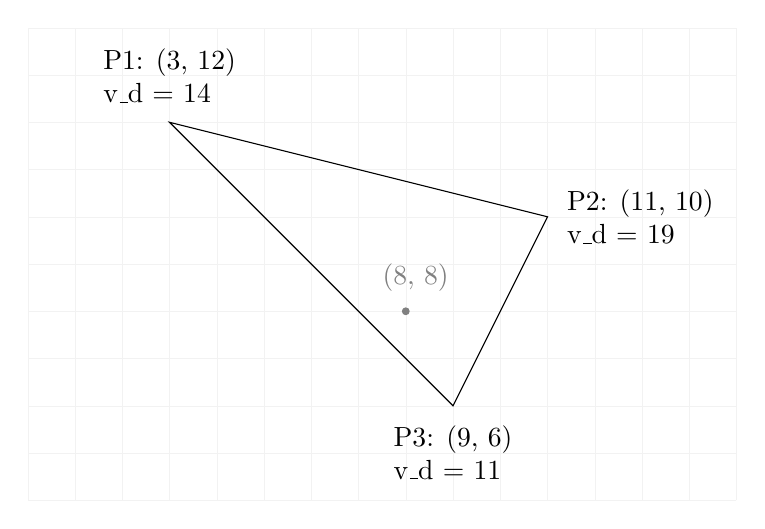
\begin{tikzpicture}[scale=0.6]
    \draw[step=1.0cm, gray!10, ultra thin](0, 4) grid (15, 14);
    \draw 
        (3, 12) node[label={[align=left]above:P1: (3, 12)\\v\_d = 14}]{} -- 
        (11, 10) node[label={[align=left]right:P2: (11, 10)\\v\_d = 19}]{} -- 
        (9,  6) node[label={[align=left]below:P3: (9, 6)\\v\_d = 11}]{} --
        cycle;
    \filldraw [gray] (8, 8) circle (2pt) node[anchor=west, label={above:(8, 8)}] {};
\end{tikzpicture}

$y_{bot} = 6$

$y_{top} = 12$

$
    x_{left}
=
    lerp\left(P3.x, P1.x, \frac{y - P3.y}{P1.y - P3.y}\right)
=
    lerp\left(9, 3, \frac{8 - 6}{12 - 6}\right)
=
    lerp\left(9, 3, \frac{1}{3}\right)
=
    9 * \left(1 - \frac{1}{3}\right) + 3 * \frac{1}{3} 
=
    6 + 1
=
    7
$

$
    x_{right}
=
    lerp\left(P3.x, P2.x, \frac{y - P3.y}{P2.y - P3.y}\right)
=
    lerp\left(9, 11, \frac{8 - 6}{10 - 6}\right)
=
    lerp\left(9, 11, \frac{1}{2}\right)
=
    9 * \left(1 - \frac{1}{2}\right) + 11 * \frac{1}{2} 
=
    4.5 + 5.5
=
    10
$

$
    v\_d_{left}
=
    lerp\left(P3.v\_d, P1.v\_d, \frac{y - P3.y}{P1.y - P3.y}\right)
=
    lerp(11, 14, \frac{1}{3})
=
    11 * \left(1 - \frac{1}{3}\right) + 14 * \frac{1}{3}
=
    12
$

$
    v\_d_{right}
=
    lerp\left(P3.v\_d, P2.v\_d, \frac{y - P3.y}{P2.y - P3.y}\right)
=
    lerp(11, 19, \frac{1}{2})
=
    11 * \left(1 - \frac{1}{2}\right) + 19 * \frac{1}{2}
=
    15
$

$
    v\_d_{pixel}
=
    lerp\left(v\_d_{left}, v\_d_{right}, \frac{x_{pixel} - x_{left}}{x_{right} - x_{left}}\right)
=
    lerp\left(12, 15, \frac{1}{3}\right)
=
    12 * \left(1 - \frac{1}{3}\right) + 15 * \frac{1}{3}
=
    13
$

Pixel (8, 8) has the v\_d value 13. Awesome!

\rule{\textwidth}{0.25mm}
A small story about the beautiful triangle image in this exercise:

Once upon a time, I was procrastinating doing this assignment. I spent some time learning how to work with geometric shaders in OpenGL and developing particle rendering concept. You know the usual weekend routine. On Monday I decided that I had to complete this to hand it in. Well... That image is the result of me procrastinating another hour and learning how to draw in \LaTeX.

I hope you have a good day sir!